\subsection{Super Puma}
\begin{figure}[h]
  \centering
  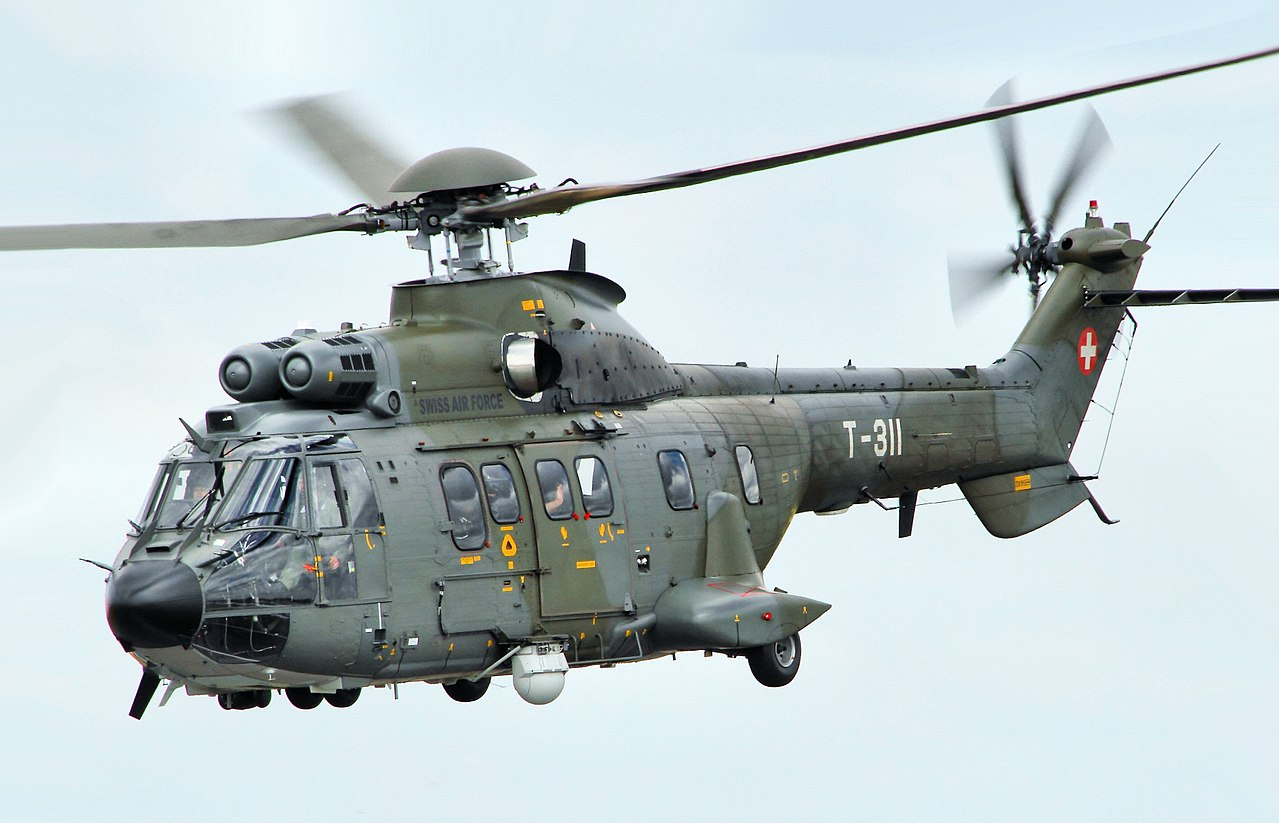
\includegraphics[width=0.7\textwidth]{images/puma.jpg}
  \caption{Ejemplo ocupando todo el ancho}
\end{figure}
El Airbus Helicopters H215 (anteriormente denominado Eurocopter AS332 Super Puma) es un helicóptero utilitario de tamaño medio, bimotor y con rotor principal de cuatro palas, diseñado a partir del SA 330 Puma. Originalmente fue fabricado por la compañía francesa Aérospatiale y después por el Grupo Eurocopter (tras la integración de Aérospatiale en el grupo europeo), que cambió de nombre a la actual Airbus Helicopters, pasando a denominarse el modelo como H215. Realizó su primer vuelo el 13 de septiembre de 1978 y fue comercializado para ser usado tanto en el ámbito civil como en el militar. Este helicóptero tiene muchas versiones, incluyendo las adaptadas para búsqueda y rescate y guerra antisubmarina. 

\subsubsection{Diseño y desarrollo}
El H215 se fabrica en dos variantes: una multiusos enfocada a operaciones muy distintas entre sí, y otra con una cabina más corta, pero con mayor capacidad para la carga de pago. Así, se distingue entre una cabina de asientos más espaciados, con 17/19 asientos, o una cabina para tropas, con 20/22 asientos; ambas opciones permiten al helicóptero operar con una carga externa de hasta 4500 kg. Además, en las últimas versiones del H215 se incorporó el autopiloto de 4 ejes empleado en el modelo militar H225, el cual aporta asistencia, precisión, estabilidad y protección en toda la envolvente de vuelo, ayudando así a mejorar la eficiencia y seguridad de las operaciones.


La versión multifunción del H215 se compone de una cabina larga y reconfigurable, un amplio rango de opciones de equipamiento, cabina del piloto compatible con gafas de visión nocturna y capacidad de actuación para todo tipo de climas. Además, cubre todo el espectro de misiones de carácter civil, ampliando el tipo de misiones que se pueden realizar de manera aérea. La versión centrada en trabajo aéreo se compone de un fuselaje más corto que la descrita anteriormente, siendo por lo general de una configuración más ligera. Así, esta versión ofrece una capacidad óptima para la carga de pago, convirtiendo el H215 en el helicóptero más empleado en materia de trabajo aéreo y extinción de incendios. Esta versión también se puede configurar para otro tipo de misiones, como el transporte de pasajeros. 
\subsubsection{Historia operacional}
En España, el H215 entró en servicio en 1982 bajo la designación del Ejército del Aire y del Espacio HD.21/HT.21. El primero de los 12 ejemplares adquiridos por el Ejército del Aire y del Espacio en 1982 llegó a la base aérea de Cuatro Vientos, Madrid, el 22 de diciembre de dicho año. De estos 12 ejemplares, 10 eran de la versión SAR y 2 en configuración VIP. Actualmente, el H215 presta servicio en el Ala 48 y en el Ala 46, concretamente en los Escuadrones 802 y 803 del SAR, y el Escuadrón 402 de transporte VIP. La familia Super Puma se empleó en misiones internacionales como la Operación India-Mike en Mozambique, en el año 2000, para aeroevacuación y distribución de ayuda humanitaria entre otras misiones. Los Super Puma correspondientes al 803 Escuadrón fueron destinados a la Base de Apoyo Avanzado de Herat, en Afganistán, para realizar misiones CSAR limitado, MEDEVAC y SASEVAC, bajo el amparo de la International Security Assistance Force (ISAF).2​


En 2018, Babcock MCS España incorporó este modelo a su flota de helicópteros en España, para la extinción de incendios forestales. Tuvo operativos 4 helicópteros; el primero en la Base de Campillo de Paraviento (Cuenca), y los restantes en las bases BRICA (brigada de refuerzo contra incendios forestales) del plan INFOCA de la Junta de Andalucía, situadas en Aznalcóllar (Sevilla), Cártama (Málaga) y Jeres del Marquesado (Granada).3​ Ese mismo año, Airbus Helicopters entregó su Super Puma número 1000 al Cuerpo de Policía alemán, que llevará a cabo misiones de salvamento marítimo.4
